\documentclass{article}
\usepackage{todonotes}
\usepackage[a4paper,margin=1in]{geometry}
\usepackage{amsmath,amssymb,amsthm,bm,mathtools}
\usepackage{graphicx}
\graphicspath{{./figures/}}
\usepackage{xcolor}
\usepackage{booktabs}
\usepackage{multirow}
\usepackage{caption}
\usepackage{subfigure}
\usepackage{authblk}
\usepackage{cite}
\usepackage[ruled,linesnumbered]{algorithm2e}
\usepackage{tikz}
\usetikzlibrary{arrows.meta,positioning,fit,calc,decorations.pathmorphing,shapes.geometric}
\usepackage[colorlinks=true,linkcolor=blue,citecolor=blue,urlcolor=blue]{hyperref}

\newtheorem{remark}{Remark}
\newtheorem{definition}{Definition}
\newtheorem{proposition}{Proposition}


\newcommand{\eps}{\varepsilon}
\newcommand{\R}{\mathbb{R}}
\newcommand{\N}{\mathbb{N}}
\newcommand{\I}{\mathbb{I}}
\newcommand{\sS}{\mathbb{S}}
\newcommand{\cA}{\mathcal{A}}
\newcommand{\cU}{\mathcal{U}}
\newcommand{\cG}{\mathcal{G}}
\newcommand{\cP}{\mathcal{P}}
\newcommand{\cB}{\mathcal{B}}
\newcommand{\cR}{\mathcal{R}}
\newcommand{\cT}{\mathcal{T}}
\newcommand{\cS}{\mathcal{S}}
\newcommand{\cK}{\mathcal{K}}
\newcommand{\cF}{\mathcal{F}}
\newcommand{\cE}{\mathcal{E}}
\newcommand{\cL}{\mathcal{L}}
\newcommand{\bx}{\bm{x}}
\newcommand{\by}{\bm{y}}
\newcommand{\bh}{\bm{h}}
\newcommand{\bp}{\bm{p}}
\newcommand{\bq}{\bm{q}}
\newcommand{\bk}{\bm{k}}
\newcommand{\bv}{\bm{v}}
\newcommand{\bw}{\bm{w}}
\newcommand{\bzero}{\bm{0}}
\newcommand{\diff}{\mathop{}\!\mathrm{d}}
\newcommand{\inner}[2]{\left\langle #1,#2\right\rangle}
\newcommand{\norm}[1]{\left\lVert #1\right\rVert}
\newcommand{\softmax}{\operatorname{softmax}}
\newcommand{\ELU}{\operatorname{ELU}}
\newcommand{\GELU}{\operatorname{GELU}}
\newcommand{\diag}{\operatorname{diag}}

\newcommand{\KW}[1]{\textcolor{purple}{{KW: #1}}}

\begin{document}
\title{Let There Be Light: Reflection, Refraction, and Scattering for Neural Operators of Parametric PDEs}

\author[]{Keke Wu}

\date{\today}

\maketitle

\begin{abstract}
Neural operators learn mappings between infinite-dimensional function spaces and provide a data-driven surrogate modeling paradigm for parametric partial differential equations. Existing architectures often obtain expressivity by either parameterizing an integral kernel in a prescribed transform domain or by applying attention directly over discretized mesh points. These designs have led to substantial progress, but they also expose a persistent tension between physical interpretability, spatial nonlocality, mesh scalability, and computational complexity. We propose a \emph{Light-inspired neural operator} (LiNO), an operator-learning architecture whose latent evolution is decomposed into three mechanisms motivated by elementary light transport: reflection, refraction, and scattering. Reflection and refraction act as adaptive feature-space transformations at each spatial location, while scattering acts as an input-dependent nonlocal spatial propagation operator. The original scattering layer is formulated as a normalized kernel map with relative positional bias, and an efficient variant replaces the quadratic pairwise kernel by a linearized global kernel plus a local diffusion branch. This yields a structured neural operator that separates local constitutive modulation from nonlocal spatial communication while remaining compatible with PDE benchmarks such as Burgers' equation, Darcy flow, and time-dependent Navier--Stokes flows. Our code is publicly available at: \url{https://github.com/wukekever/Light-inspired-neural-operator}.
\end{abstract}

\section{Introduction}

The repeated numerical solution of parametric partial differential equations (PDEs) is a central computational bottleneck in scientific computing, inverse design, uncertainty quantification, and optimal control. Given a family of PDEs indexed by input functions, coefficients, initial data, boundary data, geometry descriptors, or source terms, the central object is the solution operator
\begin{equation}
    \cG: \cA \to \cU, \qquad a \mapsto u = \cG(a),
\end{equation}
where $\cA$ and $\cU$ are function spaces. Classical numerical solvers, including finite difference, finite volume, spectral, and finite element methods, approximate each new instance by discretizing the governing equation and solving the resulting algebraic system. These methods are indispensable for reliability and accuracy, but their repeated use can be prohibitively expensive when a large number of queries is required. Neural operators address this issue by learning the entire solution map $\cG$ from data, so that a trained model can rapidly infer the solution for unseen input functions and, ideally, transfer across discretization resolutions.

Early neural-network solvers for PDEs typically learned finite-dimensional maps tied to a fixed mesh. By contrast, operator-learning methods aim to approximate mappings between function spaces. DeepONet introduced a branch--trunk decomposition motivated by universal approximation theorems for nonlinear operators \cite{lu2021deeponet}. The Fourier neural operator (FNO) parameterizes an integral kernel in Fourier space and has demonstrated resolution transfer on canonical PDE benchmarks such as Burgers' equation, Darcy flow, and Navier--Stokes equations \cite{li2021fno}. Subsequent work has expanded the design space of neural operators, including systematic comparisons and practical extensions of DeepONet and FNO \cite{lu2022comprehensive}, Laplace-domain operator parameterizations \cite{cao2023laplace}, graph- and point-cloud-based neural operators for complex geometries \cite{li2020gno,li2023pcno}, Koopman-inspired operator learning \cite{xiong2024koopman}, and transformer-based PDE solvers that use attention mechanisms to model long-range physical interactions \cite{wu2024transolver,zhou2026transolver3}. These developments have established neural operators as a promising surrogate modeling framework for PDE-governed systems.

Despite this progress, several challenges remain. First, many neural operators combine local feature mixing and nonlocal spatial propagation in a monolithic computational block, making it difficult to identify which component is responsible for local constitutive transformation, spatial transport, or long-range interaction. Second, spectral architectures such as FNO are highly efficient on regular grids but rely on a particular transform-domain inductive bias; this can be limiting for nonperiodic, localized, discontinuous, or geometry-dependent phenomena. Third, attention-based solvers provide adaptive nonlocality but the direct construction of all pairwise mesh interactions scales quadratically with the number of spatial degrees of freedom, which becomes restrictive for high-resolution PDE simulations. Finally, for a high-level scientific surrogate to be useful beyond benchmark interpolation, the architecture should expose a transparent modeling principle that can be related to physical mechanisms while still being implementable as a trainable neural operator.

This paper develops a Light-inspired neural operator (LiNO) based on a simple guiding analogy: latent feature vectors are treated as optical states, and the evolution of these states is decomposed into reflection, refraction, and scattering. The analogy is not intended to reproduce geometric optics literally. Instead, it provides a structured operator design principle. Reflection is used to model adaptive, norm-controlled redistribution of feature components; refraction is used to model anisotropic feature deformation through a learnable refractive ratio; and scattering is used to model spatial propagation through an input-dependent nonlocal kernel. In the proposed architecture, reflection and refraction act pointwise along the latent feature dimension, while scattering acts over the physical domain. This creates an explicit separation between feature-space modulation and spatial communication.

The resulting operator has three attractive properties. First, the block structure is interpretable: reflection and refraction describe local transformations of the latent physical state, whereas scattering describes nonlocal transport of information across space. Second, the architecture is flexible: it can be implemented on one-dimensional grids, two-dimensional grids, or, in principle, more general point sets by changing only the spatial scattering component. Third, the method admits both a faithful quadratic scattering layer with relative positional bias and an efficient scattering layer whose cost is linear in the number of spatial points. The efficient variant approximates the global softmax kernel by a positive feature-map factorization and restores the lost locality prior using a depthwise local diffusion branch.

The main contribution of this work is to develop a physically interpretable neural operator in which the latent solution evolution is organized by optical transport principles rather than by purely spectral or black-box transformations. Specifically, we introduce a light-inspired neural operator that decomposes feature propagation into reflection, refraction, and scattering, thereby providing a structured mechanism for local state modulation, directional feature reorientation, and nonlocal spatial information exchange. In this formulation, reflection and refraction act as adaptive pointwise transformations in the latent feature space, while scattering is realized as a nonlinear kernel operator over the physical domain. To make the framework both expressive and computationally scalable, we further present two scattering realizations: a full attention-type kernel capturing global pairwise interactions and an efficient linearized variant that couples low-rank global propagation with local diffusion. The resulting architecture admits an implementation-compatible mathematical description, including lifting, stacked light-evolution blocks, adaptive optical mixing, residual feed-forward correction, and projection, offering a unified operator-learning framework that is interpretable, modular, and extensible to diverse PDE solution-map learning tasks.



\section{Method}

\subsection{Problem setting and neural-operator formulation}

Let $\Omega \subset \R^{d_x}$ be a bounded spatial domain, with $d_x=1$ or $d_x=2$ in the present implementation (higher-dimensional extensions are straightforward). We consider a parametric PDE family whose solution operator is denoted by
\begin{equation}
    \cG: \cA \to \cU, \qquad a \mapsto u=\cG(a),
    \label{eq:operator-map}
\end{equation}
where $a:\Omega\to\R^{d_{\mathrm{in}}}$ is an input field and $u:\Omega\to\R^{d_{\mathrm{out}}}$ is the corresponding solution field. For example, $a$ may denote an initial condition for Burgers' equation, a coefficient field for Darcy flow, or an initial vorticity field for a time-dependent Navier--Stokes benchmark. The objective is to approximate $\cG$ by a parametric neural operator $\cG_\theta$.

Let $\{x_i\}_{i=1}^{N}\subset\Omega$ be a discretization of the domain. In one dimension, $N=L$; in two dimensions, $N=HW$ for a grid of size $H\times W$. The discrete input is represented in channels-last format,
\begin{equation}
    a_N = \{a(x_i)\}_{i=1}^{N} \in \R^{N\times d_{\mathrm{in}}},
\end{equation}
with the two-dimensional implementation using tensors of shape $H\times W\times d_{\mathrm{in}}$. The proposed LiNO takes the compositional form
\begin{equation}
    \cG_\theta
    =
    \Pi_\theta \circ
    \left(\cB_\theta^{(L)}\circ\cdots\circ\cB_\theta^{(1)}\right)
    \circ \cP_\theta,
    \label{eq:global-lightno}
\end{equation}
where $\cP_\theta$ is a lifting map, $\Pi_\theta$ is a projection map, and $\cB_\theta^{(\ell)}$ is the $\ell$-th light-evolution block. The latent field at layer $\ell$ is denoted by
\begin{equation}
    h^{(\ell)}:\Omega\to\R^M, \qquad
    h_i^{(\ell)} \approx h^{(\ell)}(x_i)\in\R^M,
\end{equation}
where $M$ is the latent width. In the optical analogy, $h_i^{(\ell)}$ is the latent optical state carried by the spatial location $x_i$.

The lifting and projection are pointwise affine maps,
\begin{align}
    h_i^{(0)} &= \cP_\theta(a)(x_i)=W_{\mathrm{in}} a(x_i)+b_{\mathrm{in}},
    \label{eq:lifting}\\
    \widehat{u}_i &= \Pi_\theta(h^{(L)})(x_i)=W_{\mathrm{out}}h_i^{(L)}+b_{\mathrm{out}}.
    \label{eq:projection}
\end{align}
Coordinate channels may be concatenated with the physical input field before lifting, so that the operator can distinguish spatial locations on nonperiodic domains. This is consistent with common practice in neural-operator implementations.


\subsection{Light-evolution block: reflection, refraction, and scattering}

Each light-evolution block updates the latent field through a residual rule
\begin{equation}
    h^{(\ell+1)} = h^{(\ell)} + \cE_\theta^{(\ell)}(h^{(\ell)}),
    \label{eq:residual-evolution}
\end{equation}
where $\cE_\theta^{(\ell)}$ is decomposed into three light-inspired components:
\begin{equation}
    \cE_\theta^{(\ell)}
    =
    \alpha_r^{(\ell)}\cR_\theta^{(\ell)}
    +
    \alpha_t^{(\ell)}\cT_\theta^{(\ell)}
    +
    \alpha_s^{(\ell)}\cS_\theta^{(\ell)}.
    \label{eq:light-decomposition}
\end{equation}
Here $\cR_\theta$ is reflection, $\cT_\theta$ is refraction, and $\cS_\theta$ is scattering. The reflection and refraction maps act independently at each spatial location and only mix the latent feature dimension. The scattering map operates over the physical domain and is responsible for the propagation of spatial information.

Figure~\ref{fig:light-block} illustrates the block structure. The input latent state is normalized and sent through three branches. Reflection and refraction transform each feature vector locally, while scattering constructs a spatial propagation operator. The three outputs are combined by adaptive mixture weights and passed through a residual projection and pointwise feed-forward correction.

\begin{figure}[t]
\centering
\resizebox{0.96\textwidth}{!}{
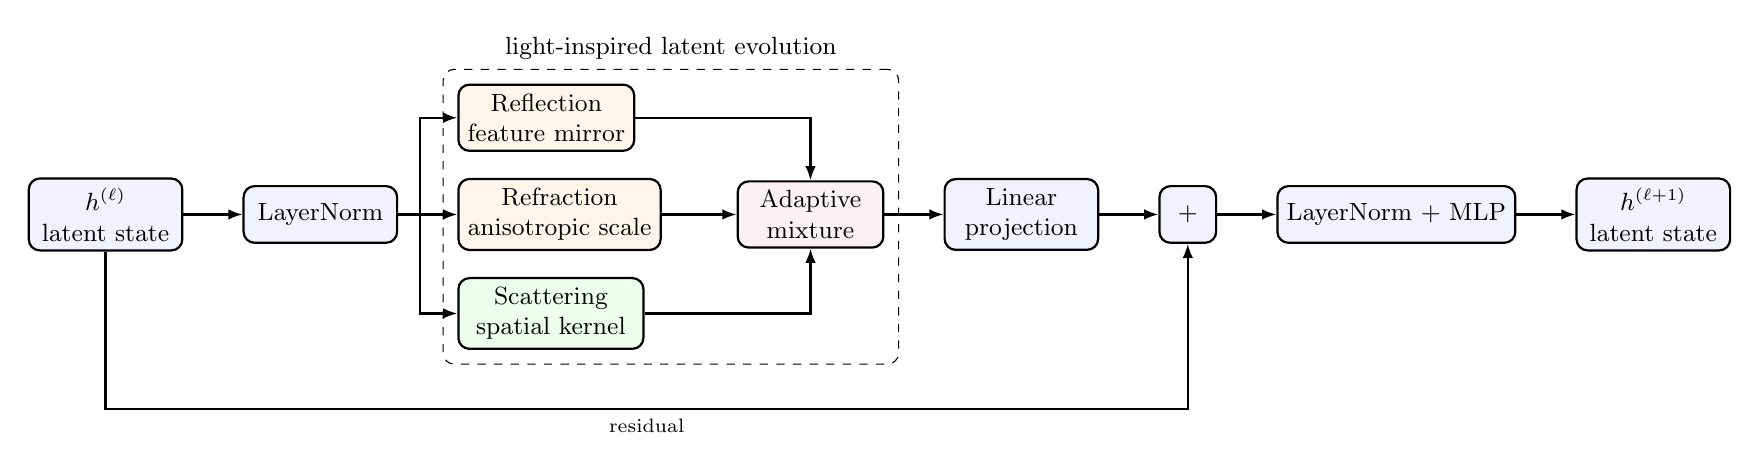
\begin{tikzpicture}[
    node distance=0.65cm and 0.75cm,
    box/.style={draw, rounded corners, thick, align=center, minimum height=0.72cm, minimum width=1.95cm, fill=blue!5, font=\small},
    op/.style={draw, rounded corners, thick, align=center, minimum height=0.72cm, minimum width=2.20cm, fill=orange!8, font=\small},
    scat/.style={draw, rounded corners, thick, align=center, minimum height=0.72cm, minimum width=2.35cm, fill=green!8, font=\small},
    small/.style={draw, rounded corners, thick, align=center, minimum height=0.68cm, minimum width=1.85cm, fill=purple!6, font=\small},
    arr/.style={-{Latex[length=1.8mm]}, thick}
]

\node[box] (input) {$h^{(\ell)}$\\latent state};
\node[box, right=of input] (norm) {LayerNorm};
\node[op, above right=0.42cm and 0.75cm of norm] (reflect) {Reflection\\feature mirror};
\node[op, right=0.75cm of norm] (refract) {Refraction\\anisotropic scale};
\node[scat, below right=0.42cm and 0.75cm of norm] (scatter) {Scattering\\spatial kernel};
\node[small, right=0.95cm of refract] (mix) {Adaptive\\mixture};
\node[box, right=of mix] (proj) {Linear\\projection};
\node[box, right=of proj, minimum width=0.72cm] (res1) {$+$};
\node[box, right=of res1] (ffn) {LayerNorm + MLP};
\node[box, right=of ffn] (output) {$h^{(\ell+1)}$\\latent state};

\draw[arr] (input) -- (norm);
\draw[arr] (norm.east) -- ++(0.28,0) |- (reflect.west);
\draw[arr] (norm) -- (refract);
\draw[arr] (norm.east) -- ++(0.28,0) |- (scatter.west);
\draw[arr] (reflect.east) -| (mix.north);
\draw[arr] (refract.east) -- (mix.west);
\draw[arr] (scatter.east) -| (mix.south);
\draw[arr] (mix) -- (proj);
\draw[arr] (proj) -- (res1);
% \draw[arr] (input.south) to[out=-70,in=-110] node[below,sloped,font=\scriptsize]{residual} (res1.south);
\draw[arr]
    (input.south) -- ++(0,-2.00)
    -| node[pos=0.25, below, font=\scriptsize]{residual} (res1.south);
\draw[arr] (res1) -- (ffn);
\draw[arr] (ffn) -- (output);

\node[
    draw,
    dashed,
    rounded corners,
    fit=(reflect)(refract)(scatter)(mix),
    inner sep=0.18cm,
    label={[font=\small]above:{light-inspired latent evolution}}
] {};
\end{tikzpicture}
}
\caption{Schematic of a LiNO evolution block. Reflection and refraction are pointwise transformations along the latent feature dimension, whereas scattering propagates information over the spatial domain through a learned kernel. The three branches are combined by input-dependent mixture weights.}
\label{fig:light-block}
\end{figure}

\subsection{Reflection: adaptive feature-space mirror transformation}

In physical optics, reflection changes the direction of propagation according to the local interface normal. In LiNO, we reinterpret this mechanism in feature space: the latent vector $h_i\in\R^M$ at each spatial point is reflected with respect to an adaptive hyperplane whose normal direction is learned from the current state.

For each spatial index $i$, define an adaptive direction
\begin{equation}
    v_i = W_r h_i + b_r, \qquad
    \widehat{v}_i = \frac{v_i}{\norm{v_i}_2},
    \label{eq:adaptive-normal}
\end{equation}
where $W_r\in\R^{M\times M}$ and $b_r\in\R^M$ are trainable parameters. The reflection operator is given by the Householder-type formula
\begin{equation}
    \cR_\theta(h_i)
    =
    h_i - 2\inner{h_i}{\widehat{v}_i}\widehat{v}_i.
    \label{eq:reflection}
\end{equation}
For a fixed unit direction $\widehat v_i$, this transformation is equivalent to applying the Householder matrix
\begin{equation}
    H_i = I_M - 2\widehat v_i \widehat v_i^\top
\end{equation}
to the feature vector $h_i$, namely
\begin{equation}
    \cR_\theta(h_i)=H_i h_i.
\end{equation}
A direct implementation of this matrix-vector product would require forming the dense matrix
$H_i\in\R^{M\times M}$, leading to $O(M^2)$ storage and computational cost per spatial location. In contrast, we use the matrix-free Householder identity in \eqref{eq:reflection}: the reflection is computed only through one inner product
$\inner{h_i}{\widehat v_i}$ and one rank-one rescaling of $\widehat v_i$. Consequently, the cost of the reflection step is reduced to $O(M)$ per spatial point, while retaining the exact action of the corresponding Householder reflection.

Geometrically, \eqref{eq:reflection} reverses the component of $h_i$ along $\widehat v_i$ while keeping the tangential component unchanged. Indeed, writing
\begin{equation}
    h_i^{\perp}=\inner{h_i}{\widehat v_i}\widehat v_i,
    \qquad
    h_i^{\parallel}=h_i-h_i^{\perp},
\end{equation}
we obtain
\begin{equation}
    \cR_\theta(h_i)=h_i^{\parallel}-h_i^{\perp}.
\end{equation}
Thus, reflection provides a learnable, direction-dependent redistribution of latent features without introducing cross-site spatial coupling. This is useful when the input field induces sharp changes, interfaces, or local directional modes, because the model can locally reorient the latent representation before applying spatial propagation.

\subsection{Refraction: anisotropic feature deformation}

Refraction describes the change of propagation direction when light crosses an interface between two media with different refractive indices. In geometric optics, the incident and transmitted directions are related by Snell's law,
\begin{equation}
    n_1 \sin \alpha_1 = n_2 \sin \alpha_2,
\end{equation}
where $n_1,n_2$ are the refractive indices of the two media, and $\alpha_1,\alpha_2$ are the angles measured with respect to the interface normal. The essential implication is that a change of medium induces an anisotropic modification of the propagation state: the component associated with the interface normal is altered, while the tangential component is constrained by the transmission condition.

Motivated by this principle, LiNO interprets refraction as a local anisotropic deformation of the latent feature vector. Instead of explicitly solving a geometric-optics transmission problem in the physical space, we introduce an adaptive feature-space normal and use it to separate the latent state into tangential and normal components. Using the same form of adaptive direction as in \eqref{eq:adaptive-normal}, but with independent trainable parameters, we define
\begin{equation}
    h_i=h_i^{\parallel}+h_i^{\perp},
    \qquad
    h_i^{\perp}=\inner{h_i}{\widehat v_i}\widehat v_i,
    \qquad
    h_i^{\parallel}=h_i-h_i^{\perp}.
\end{equation}
The refraction operator is then defined by
\begin{equation}
    \cT_\theta(h_i)
    =
    h_i^{\parallel}+\eta h_i^{\perp},
    \label{eq:refraction}
\end{equation}
where $\eta$ is a learnable refractive factor. This construction can be viewed as a simplified Snell-type transformation in latent space: the tangential component $h_i^{\parallel}$ is preserved, while the normal component $h_i^{\perp}$ is rescaled according to a learned refractive contrast. Thus, $\eta$ plays the role of an effective refractive-index ratio, controlling how strongly the latent state is bent or compressed along the adaptive normal direction.

Equivalently, for a fixed unit vector $\widehat v_i$, \eqref{eq:refraction} can be written as
\begin{equation}
    \cT_\theta(h_i)
    =
    \left(I_M + (\eta-1)\widehat v_i \widehat v_i^\top\right)h_i.
    \label{eq:refraction-matrix}
\end{equation}
A direct implementation of \eqref{eq:refraction-matrix} would require forming and applying a dense feature-space matrix in $\R^{M\times M}$, resulting in $O(M^2)$ cost per spatial location. We instead use the matrix-free decomposition in \eqref{eq:refraction}: the operator is evaluated through one inner product and one rank-one rescaling along $\widehat v_i$. Consequently, the refraction step costs only $O(M)$ per spatial point while retaining the exact action of the corresponding rank-one anisotropic deformation.

In the implementation, the refractive factor is constrained near unity by
\begin{equation}
    \eta = 1 + \rho\tanh(\gamma),
    \label{eq:eta-param}
\end{equation}
where $\gamma$ is trainable and $\rho>0$ is a prescribed range parameter. This parameterization has two purposes. First, it initializes the refraction layer close to the identity map, preventing excessive distortion of the latent representation at the beginning of training. Second, it bounds the local amplification and attenuation induced by refraction, which improves the stability of deep compositions of light-evolution blocks.

Reflection and refraction are complementary. Reflection flips a selected feature component and is approximately norm-preserving when $\widehat v_i$ is normalized, whereas refraction continuously rescales that component. Consequently, reflection provides a discrete geometric reorientation, while refraction provides a smooth anisotropic modulation. Both operations are pointwise in $x$, so they do not replace spatial propagation; rather, they reshape the latent state locally before and after nonlocal scattering.

\subsection{Scattering as nonlinear spatial kernel propagation}

Scattering is the only component that explicitly couples different spatial locations. Its role is to propagate latent information over the domain through a normalized, input-dependent kernel. Let $h_i\in\R^M$ denote the latent state at $x_i$. We first define query, key, and value embeddings
\begin{equation}
    q_i=W_q h_i,
    \qquad
    k_i=W_k h_i,
    \qquad
    z_i=W_v h_i,
    \label{eq:qkv}
\end{equation}
where $W_q,W_k\in\R^{d\times M}$ and $W_v\in\R^{M\times M}$ are trainable matrices. The standard scattering kernel is
\begin{equation}
    K_{ij}
    =
    \frac{
    \exp\left(d^{-1/2}q_i^\top k_j + b_{ij}\right)
    }{
    \sum_{m=1}^{N}\exp\left(d^{-1/2}q_i^\top k_m + b_{im}\right)
    },
    \label{eq:standard-kernel}
\end{equation}
where $b_{ij}$ is a relative positional bias. For a regular grid, normalized coordinates $p_i\in[0,1]^{d_x}$ are assigned to each spatial location and
\begin{equation}
    b_{ij}=-\tau\norm{p_i-p_j}_2^2,
    \qquad \tau=\operatorname{softplus}(\tau_0)>0.
    \label{eq:relative-bias}
\end{equation}
The parameter $\tau$ controls the locality of the scattering kernel: larger values favor short-range interaction, whereas smaller values allow more global mixing.

The standard scattering update is
\begin{equation}
    (\cS_\theta h)_i
    =
    \sigma_s\left(\sum_{j=1}^{N}K_{ij}z_j-h_i\right),
    \qquad
    \sigma_s=\exp(\lambda_s)>0.
    \label{eq:standard-scattering}
\end{equation}
Because $K_{ij}$ is row-stochastic,
\begin{equation}
    \sum_{j=1}^{N}K_{ij}=1,
\end{equation}
\eqref{eq:standard-scattering} can be interpreted as a relaxation between the current state and a kernel-weighted spatial average. It resembles graph diffusion, collision--scattering relaxation, and nonlocal integral propagation, but with a kernel that depends on the latent field. In the continuum limit, the formal analogue is
\begin{equation}
    (\cS_\theta h)(x)
    =
    \sigma_s\left(
    \int_{\Omega}K_\theta(x,y;h)Z_\theta h(y)\,\diff y - h(x)
    \right),
    \label{eq:continuum-scattering}
\end{equation}
where $Z_\theta$ denotes the value projection and $K_\theta$ is a nonlinear normalized kernel.

\begin{algorithm}[t]
\caption{Standard scattering layer with relative positional bias}
\label{alg:standard-scattering}
\KwIn{Latent field $h\in\R^{B\times N\times M}$; normalized coordinates $p_i\in[0,1]^{d_x}$}
\KwOut{Scattering residual $s\in\R^{B\times N\times M}$}
Compute $q=W_qh$, $k=W_kh$, $z=W_vh$\;
Compute pairwise distances $D_{ij}=\norm{p_i-p_j}_2^2$\;
Set $A_{ij}=d^{-1/2}q_i^\top k_j-\operatorname{softplus}(\tau_0)D_{ij}$\;
Normalize $K_{ij}=\softmax_j(A_{ij})$\;
Compute $y_i=\sum_{j=1}^{N}K_{ij}z_j$\;
Return $s_i=\exp(\lambda_s)(y_i-h_i)$\;
\end{algorithm}

The standard implementation in Algorithm~\ref{alg:standard-scattering} requires forming the dense matrix $K\in\R^{N\times N}$. Therefore, its memory and computational cost scale as $\mathcal{O}(N^2)$ up to channel factors. This is acceptable for moderate grids, but it becomes a bottleneck for high-resolution PDE simulation.

\subsection{Efficient scattering: linearized global kernel plus local diffusion}

To improve scalability, we replace the full softmax kernel by a linearized positive-kernel approximation. The key idea is to approximate the exponential dot-product kernel by a separable feature map
\begin{equation}
    \exp(q_i^\top k_j)
    \approx
    \phi(q_i)^\top \phi(k_j),
    \label{eq:feature-map-approx}
\end{equation}
where $\phi:\R^d\to\R_+^d$ is positive. In the implementation, we use
\begin{equation}
    \phi(z)=\ELU(z)+1,
    \label{eq:elu-feature-map}
\end{equation}
which is simple, positive, and numerically stable.

Because the explicit pairwise positional bias in \eqref{eq:relative-bias} would reintroduce an $N^2$ matrix, efficient scattering injects spatial information through a coordinate encoder instead. Let
\begin{equation}
    c_i = C_\theta(p_i)\in\R^d
\end{equation}
be a learnable coordinate embedding implemented by a small multilayer perceptron. The efficient queries and keys are
\begin{equation}
    \widetilde q_i=d^{-1/2}W_qh_i+c_i,
    \qquad
    \widetilde k_i=d^{-1/2}W_kh_i+c_i.
    \label{eq:coord-qk}
\end{equation}
The global linear attention output is then
\begin{equation}
    y_i^{\mathrm{glob}}
    =
    \frac{
    \phi(\widetilde q_i)^\top
    \left(\sum_{j=1}^{N}\phi(\widetilde k_j)z_j^\top\right)
    }{
    \phi(\widetilde q_i)^\top
    \left(\sum_{j=1}^{N}\phi(\widetilde k_j)\right)
    }.
    \label{eq:linear-attention}
\end{equation}
Equivalently, define the global statistics
\begin{equation}
    A=\sum_{j=1}^{N}\phi(\widetilde k_j)z_j^\top\in\R^{d\times M},
    \qquad
    s=\sum_{j=1}^{N}\phi(\widetilde k_j)\in\R^d.
\end{equation}
Then
\begin{equation}
    y_i^{\mathrm{glob}}
    =
    \frac{\phi(\widetilde q_i)^\top A}{\phi(\widetilde q_i)^\top s}.
\end{equation}
This formulation avoids constructing pairwise interactions and has cost $\mathcal{O}(NdM)$ for a single sample.

The linearized global kernel captures long-range communication but does not explicitly retain the Gaussian locality prior in \eqref{eq:relative-bias}. We therefore add a local diffusion branch
\begin{equation}
    y^{\mathrm{loc}} = P_{\mathrm{loc}}\left(D_{\mathrm{dw}}h\right),
    \label{eq:local-branch}
\end{equation}
where $D_{\mathrm{dw}}$ is a depthwise convolution over the physical grid and $P_{\mathrm{loc}}$ is a pointwise linear projection. In one dimension $D_{\mathrm{dw}}$ is a depthwise one-dimensional convolution; in two dimensions it is a depthwise two-dimensional convolution. The branch is a lightweight surrogate for local scattering and diffusion.

The final efficient scattering average combines global and local contributions:
\begin{equation}
    y_i=(1-\beta)y_i^{\mathrm{glob}}+\beta y_i^{\mathrm{loc}},
    \qquad
    \beta=\operatorname{sigmoid}(\gamma_{\mathrm{loc}})\in(0,1),
    \label{eq:hybrid-scattering-output}
\end{equation}
followed by the scattering residual
\begin{equation}
    (\cS_\theta h)_i=\exp(\lambda_s)(y_i-h_i).
    \label{eq:efficient-scattering}
\end{equation}
This decomposition approximates the original nonlocal kernel by
\begin{equation}
    \cK_\theta
    \approx
    \cK_\theta^{\mathrm{glob}}+\cK_\theta^{\mathrm{loc}},
    \label{eq:kernel-decomp}
\end{equation}
where $\cK_\theta^{\mathrm{glob}}$ is a low-rank global propagation operator and $\cK_\theta^{\mathrm{loc}}$ is a local diffusion-like operator.

\begin{algorithm}[t]
\caption{Efficient scattering layer}
\label{alg:efficient-scattering}
\KwIn{Latent field $h\in\R^{B\times N\times M}$; normalized coordinates $p_i\in[0,1]^{d_x}$}
\KwOut{Efficient scattering residual $s\in\R^{B\times N\times M}$}
Compute $z=W_vh$ and coordinate embeddings $c_i=C_\theta(p_i)$\;
Set $\widetilde q_i=d^{-1/2}W_qh_i+c_i$ and $\widetilde k_i=d^{-1/2}W_kh_i+c_i$\;
Compute positive features $Q_i=\ELU(\widetilde q_i)+1$, $K_i=\ELU(\widetilde k_i)+1$\;
Aggregate $A=\sum_{j=1}^{N}K_jz_j^\top$ and $s_K=\sum_{j=1}^{N}K_j$\;
Compute $y_i^{\mathrm{glob}}=(Q_i^\top A)/(Q_i^\top s_K)$\;
Compute local branch $y^{\mathrm{loc}}=P_{\mathrm{loc}}(D_{\mathrm{dw}}h)$\;
Mix $y_i=(1-\beta)y_i^{\mathrm{glob}}+\beta y_i^{\mathrm{loc}}$, where $\beta=\operatorname{sigmoid}(\gamma_{\mathrm{loc}})$\;
Return $s_i=\exp(\lambda_s)(y_i-h_i)$\;
\end{algorithm}

The efficient scattering layer reduces the dominant spatial complexity from quadratic to linear in $N$:
\begin{equation}
    \mathrm{standard:}\quad \mathcal{O}(N^2(d+M)),
    \qquad
    \mathrm{efficient:}\quad \mathcal{O}(NdM)+\mathcal{O}(NkM),
\end{equation}
where $k$ is the local convolution stencil size. For high-resolution grids, this is the difference between explicitly modeling all pairwise spatial interactions and summarizing them through global kernel statistics plus a local propagation correction.

\subsection{Adaptive mixture of light components}

The relative importance of reflection, refraction, and scattering should depend on the input instance and on the latent state. For example, a coefficient field with sharp inclusions may benefit from stronger local feature reorientation, while a smooth global flow field may require stronger nonlocal propagation. LiNO therefore uses adaptive mixture weights.

Let
\begin{equation}
    \overline h
    =
    \frac{1}{N}\sum_{i=1}^{N}h_i\in\R^M
    \label{eq:global-pool}
\end{equation}
be the spatially averaged latent state. A small gating network $g_\theta:\R^M\to\R^3$ produces
\begin{equation}
    (\alpha_r,\alpha_t,\alpha_s)
    =
    \softmax(g_\theta(\overline h)).
    \label{eq:gating}
\end{equation}
Thus
\begin{equation}
    \alpha_r+\alpha_t+\alpha_s=1,
    \qquad
    \alpha_r,\alpha_t,\alpha_s\ge 0.
\end{equation}
The branch mixture is
\begin{equation}
    m_i
    =
    \alpha_r\cR_\theta(h_i)
    +
    \alpha_t\cT_\theta(h_i)
    +
    \alpha_s(\cS_\theta h)_i.
    \label{eq:branch-mixture}
\end{equation}
The full block then applies a linear residual projection and a pointwise feed-forward correction:
\begin{align}
    \widetilde h_i &= h_i + W_o m_i,
    \label{eq:out-proj}\\
    h_i^+ &= \widetilde h_i + \operatorname{MLP}_\theta(\operatorname{LN}(\widetilde h_i)).
    \label{eq:ffn-correction}
\end{align}
Layer normalization is applied before the light branches and before the feed-forward network. This choice is consistent with stable residual architectures and improves the conditioning of the learned latent evolution.


\section{Experiments}

\subsection{Experimental setup}

We evaluate the proposed Light-inspired Neural Operator (LiNO) on representative one-dimensional and two-dimensional PDE benchmarks, including Burgers' equation, Darcy flow, and two-dimensional Navier--Stokes dynamics. All datasets are stored in MATLAB format and converted to channel-last PyTorch tensors before training. For a one-dimensional field, the input tensor has shape
\begin{equation}
    B\times L\times d_{\mathrm{in}},
\end{equation}
whereas for a two-dimensional field it has shape
\begin{equation}
    B\times H\times W\times d_{\mathrm{in}}.
\end{equation}
The lifting map sends the last dimension to width $M$, the stacked light-evolution blocks preserve the spatial shape and latent width, and the projection map maps the latent representation to $d_{\mathrm{out}}$ output channels.

Unless otherwise stated, we use latent width $M=128$ and stack $8$ light-evolution blocks. The efficient scattering layer is used as the default scattering module, while the full pairwise scattering layer is retained as a reference implementation for ablation and small-resolution experiments. Burgers' equation is modeled by a one-dimensional LiNO, whereas Darcy flow and Navier--Stokes dynamics are modeled by a two-dimensional LiNO. The same light-evolution block is used across all benchmarks; only the data interface, spatial dimension, input/output channels, and training protocol are changed.

For all benchmarks, the data are randomly permuted using a fixed seed before splitting. We apply unit Gaussian normalization to the physical input channels and target fields using statistics computed from the training set. Coordinate channels, when used, are concatenated to the physical input channels and are not normalized. The relative error is computed sample-wise by flattening all spatial and channel dimensions and then averaging over the mini-batch.

\subsection{Training objective}

Given training pairs $\{(a^{(n)},u^{(n)})\}_{n=1}^{N_{\mathrm{train}}}$, LiNO is trained by minimizing a composite field-matching objective that combines the mean-square error and the relative $L^2$ error. For stationary or single-shot operator learning tasks, such as coefficient-to-solution maps, we use
\begin{equation}
    \mathcal{J}(\theta)
    =
    \frac{1}{N_{\mathrm{train}}}
    \sum_{n=1}^{N_{\mathrm{train}}}
    \left[
    \lambda_{\mathrm{mse}}
    \norm{\mathcal{G}_{\theta}(a^{(n)})-u^{(n)}}_2^2
    +
    \lambda_{\mathrm{rel}}
    \frac{
    \norm{\mathcal{G}_{\theta}(a^{(n)})-u^{(n)}}_2
    }{
    \norm{u^{(n)}}_2
    }
    \right],
    \label{eq:training-loss}
\end{equation}
where $\lambda_{\mathrm{mse}}=\lambda_{\mathrm{rel}}=1$ and $\varepsilon_{\mathrm{loss}}=10^{-12}$ in the current implementation. The MSE term penalizes pointwise field discrepancies and provides stable gradient information, while the relative $L^2$ term measures the scale-normalized prediction error commonly reported in neural-operator benchmarks.

For autoregressive time-dependent prediction, we additionally include step-wise rollout errors. Let $\widehat u_{t_m:t_{m+s}}$ and $u_{t_m:t_{m+s}}$ denote the predicted and reference solution segments over the $m$-th output window. The autoregressive relative loss is
\begin{equation}
    \mathcal{J}_{\mathrm{ar}}(\theta)
    =
    \sum_{m=0}^{K-1}
    \frac{
    \norm{\widehat u_{t_m:t_{m+s}}-u_{t_m:t_{m+s}}}_2
    }{
    \norm{u_{t_m:t_{m+s}}}_2
    },
    \label{eq:ar-relative-loss}
\end{equation}
and the full rollout objective is
\begin{equation}
    \mathcal{J}_{\mathrm{rollout}}(\theta)
    =
    \lambda_{\mathrm{mse}}
    \norm{\widehat u_{1:T}-u_{1:T}}_2^2
    +
    \lambda_{\mathrm{ar}}
    \mathcal{J}_{\mathrm{ar}}(\theta),
    \label{eq:rollout-loss}
\end{equation}
with $\lambda_{\mathrm{mse}}=\lambda_{\mathrm{ar}}=1$.

\subsection{Optimization and evaluation}

All models are trained with the AdamW optimizer with initial learning rate $\eta_0=10^{-3}$ and weight decay $10^{-5}$. We use a step learning-rate scheduler that multiplies the learning rate by $0.96$ every $5$ epochs. The batch size is set to $4$ for all benchmarks, and training is performed for $500$ epochs unless otherwise specified. Gradient clipping with maximum norm $1.0$ is applied after backpropagation to improve stability. The random seed is fixed to $42$ for data splitting and model training.



































\section{Conclusion}

We have presented the formulation of a Light-inspired neural operator for parametric PDEs. The proposed method decomposes latent evolution into reflection, refraction, and scattering, thereby separating local feature transformation from nonlocal spatial propagation. The standard scattering layer realizes a normalized nonlinear kernel with relative positional bias, whereas the efficient scattering layer combines positive-feature linear attention with a local diffusion branch. This construction provides a mathematically transparent and implementation-ready neural-operator architecture for one- and two-dimensional PDE surrogate modeling.









\begin{thebibliography}{99}

\bibitem{lu2021deeponet}
L.~Lu, P.~Jin, and G.~E. Karniadakis.
\newblock Learning nonlinear operators via DeepONet based on the universal approximation theorem of operators.
\newblock \emph{Nature Machine Intelligence}, 3:218--229, 2021.

\bibitem{li2021fno}
Z.~Li, N.~Kovachki, K.~Azizzadenesheli, B.~Liu, K.~Bhattacharya, A.~Stuart, and A.~Anandkumar.
\newblock Fourier neural operator for parametric partial differential equations.
\newblock In \emph{International Conference on Learning Representations}, 2021.

\bibitem{lu2022comprehensive}
L.~Lu, X.~Meng, S.~Cai, Z.~Mao, S.~Goswami, Z.~Zhang, and G.~E. Karniadakis.
\newblock A comprehensive and fair comparison of two neural operators (with practical extensions) based on FAIR data.
\newblock \emph{Computer Methods in Applied Mechanics and Engineering}, 393:114778, 2022.

\bibitem{cao2023laplace}
Q.~Cao, S.~Goswami, and G.~E. Karniadakis.
\newblock LNO: Laplace neural operator for solving differential equations.
\newblock \emph{arXiv preprint arXiv:2303.10528}, 2023.

\bibitem{li2020gno}
Z.~Li, N.~Kovachki, K.~Azizzadenesheli, B.~Liu, K.~Bhattacharya, A.~Stuart, and A.~Anandkumar.
\newblock Neural operator: Graph kernel network for partial differential equations.
\newblock \emph{arXiv preprint arXiv:2003.03485}, 2020.

\bibitem{li2023pcno}
C.~Zeng, Y.~Zhang, J.~Zhou, Y.~Wang, Z.~Wang, Y.~Liu, L.~Wu, and D.~Z. Huang.
\newblock Point cloud neural operator for parametric PDEs on complex and variable geometries.
\newblock \emph{Computer Methods in Applied Mechanics and Engineering}, 443:118022, 2025.

\bibitem{xiong2024koopman}
W.~Xiong, X.~Huang, Z.~Zhang, R.~Deng, P.~Sun, and Y.~Tian.
\newblock Koopman neural operator as a mesh-free solver of nonlinear partial differential equations.
\newblock \emph{Journal of Computational Physics}, 113194, 2024.

\bibitem{wu2024transolver}
H.~Wu, H.~Luo, H.~Wang, J.~Wang, and M.~Long.
\newblock Transolver: A fast transformer solver for PDEs on general geometries.
\newblock In \emph{International Conference on Machine Learning}, 2024.

\bibitem{zhou2026transolver3}
H.~Zhou, H.~Wu, H.~Shangguan, Y.~Ma, H.~Weng, J.~Wang, and M.~Long.
\newblock Transolver-3: Scaling up transformer solvers to industrial-scale geometries.
\newblock \emph{arXiv preprint arXiv:2602.04940}, 2026.

\bibitem{vaswani2017attention}
A.~Vaswani, N.~Shazeer, N.~Parmar, J.~Uszkoreit, L.~Jones, A.~N. Gomez, L.~Kaiser, and I.~Polosukhin.
\newblock Attention is all you need.
\newblock In \emph{Advances in Neural Information Processing Systems}, 2017.

\bibitem{katharopoulos2020transformers}
A.~Katharopoulos, A.~Vyas, N.~Pappas, and F.~Fleuret.
\newblock Transformers are RNNs: Fast autoregressive transformers with linear attention.
\newblock In \emph{International Conference on Machine Learning}, 2020.

\end{thebibliography}

\end{document}
